\begin{frame}{El recaudo del IVA aumentó cerca de 0,1 puntos del PIB en 2025}
\centering
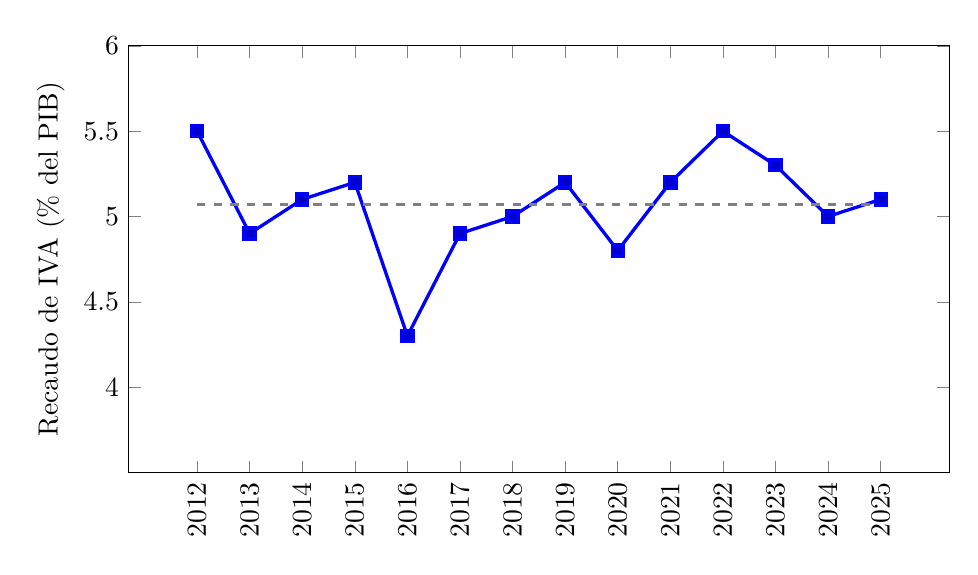
\begin{tikzpicture}
\begin{axis}[
    width=12cm,
    height=7cm,
    ylabel={Recaudo de IVA (\% del PIB)},
    ymin=3.5,ymax=6,
    ytick={4,4.5,5,5.5,6},
    xtick={2012,2013,...,2025},
    xticklabel style={rotate=90,anchor=east,/pgf/number format/.cd,1000 sep={}}
]
\addplot+[mark=square*,solid,very thick] coordinates {
(2012,5.5) (2013,4.9) (2014,5.1) (2015,5.2) (2016,4.3) (2017,4.9)
(2018,5.0) (2019,5.2) (2020,4.8) (2021,5.2) (2022,5.5) (2023,5.3)
(2024,5.0) (2025,5.1)
};
\addplot[dashed,thick,gray] coordinates {(2012,5.07) (2025,5.07)};
\end{axis}
\end{tikzpicture}
\scriptsize El valor de 2025 es una aproximación: suma la contribución de 0,1 puntos reportada por el MFMP al nivel de 2024.
\note{[Sources] MFMP 2026, capítulo 1, gráfico 1.5. Serie 2012-2024: Balance Fiscal del GNC, como en la versión fuente.}
\end{frame}